\documentclass[a4paper, 12pt]{article}
\usepackage[utf8]{inputenc}
\usepackage[english,russian]{babel}
\usepackage[warn]{mathtext}
\usepackage{graphicx}
\usepackage{float}
\usepackage{multirow}
\restylefloat{table}
\usepackage{amsmath}
\usepackage{floatflt}
\usepackage[T2A]{fontenc}
\usepackage[left=20mm, top=20mm, right=20mm, bottom=20mm, footskip=10mm]{geometry}

\tolerance 1414
\hbadness 1414
\emergencystretch 1.5em
\hfuzz 0.3pt        % размер максимального переполнения без warning'a
\widowpenalty=10000 % запрещает одиночную строку абзаца в начале страницы
\vfuzz \hfuzz
\raggedbottom       % если на странице мало содержимого, добавить пустое место в конце, а не в середине страницы



\begin{document}

\begin{titlepage}
	\centering
	\vspace{5cm}
	{\scshape\LARGE московский физико-технический институт (национальный исследовательский университет) \par}
	\vspace{6cm}
	{\scshape\Large Лабораторная работа 1.3 \par}
	{\huge\bfseries Эффект Рамзауэра \par}
	\vspace{1cm}
	\vfill
\begin{flushright}
	{\large Б03-104}\par
	\vspace{0.3cm}
	{\LARGE Куланов Александр}
\end{flushright}
	

	\vfill


	Долгопрудный, 2023 г.
\end{titlepage}

\begin{itemize}
	\item \textbf{Цель работы:} исследовать энергетическую зависимость вероятности рассеяния электронов атомами ксенона, определить энергии электронов, при которых наблюдается "просветление" ксенона, и оценить размер его внешней электронной оболочки.
\end{itemize}

\section{Теоретические сведения}

Эффективное сечение реакции -- величина, характеризующая вероятность перехода системы двух сталкивающихся 
частиц в результате их рассеяния (упругого или неупругого) в определенное конечное состояние. 
Сечение $ \sigma $ равно отношению числа $ N $ таких переходов в единицу времени к плотности потока рассеиваемых 
частиц $ n v $, падающих на мишень, т. е. к числу частиц, проходящих в единицу времени через единичную площадку, 
перпендикулярную к их скорости $ v $ ($ n $ -- плотность числа падающих частиц).

\begin{equation}\label{eq:sigma}
	\sigma = \frac{N}{n v}.
\end{equation}
Таким образом, сечение имеет размерность площади.
\begin{figure}[H]
	\centering
	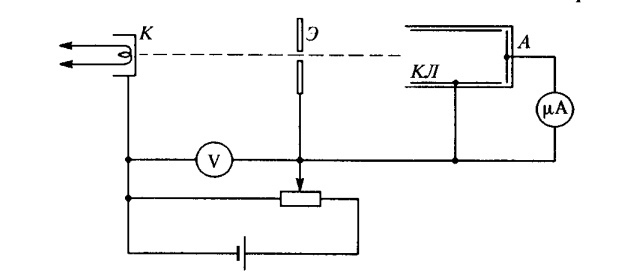
\includegraphics[width=0.5\linewidth]{fig_1.jpg}
	\caption{Схема установки для измерения сечения рассеяния электронов в газах}
	\label{fig:screenshot2}
\end{figure}
По мере уменьшения энергии электрона от нескольких десятков электрон-вольт поперечное сечение его упругого рассеяния растет. 
Однако при энергиях меньше 16 эВ в случае аргона сечение начинает уменьшаться, а при $ E \sim 1 $ эВ практически равно нулю, т. е. аргон становится прозрачным для электронов. 
При дальнейшем уменьшении энергии электронов сечение рассеяния опять начинает возрастать. Это поведение поперечного сечения свойственно не только атомам аргона, но и атомам всех инертных газов. 
Такое поведение электронов нельзя объяснить с позиций классической физики. Объяснение этого эффекта потребовало учета волновой природы электронов. Схема эксперимента Рамзауэра показана, на рис. 1.


С точки зрения квантовой теории, внутри атома потенциальная энергия налетающего электрона $ U $ отлична от нуля, скорость электрона изменяется, становясь равной $ v' $ в соответствии с законом сохранения энергии
\begin{equation*}
	E = \frac{m v^2}{2} = \frac{m v'^2}{2}+ U,
\end{equation*}
а значит, изменяется и длина его волны де Бройля. Таким образом, по отношению к электронной волне атом ведет себя как преломляющая среда с относительным показателем преломления
\begin{equation*}
	n = \frac{\lambda}{\lambda'} = \sqrt{1-\frac{U}{E}}.
\end{equation*}

Коэффициент прохождения электронов максимален при условии
\begin{equation}\label{eq:at}
	\sqrt{\frac{2 m (E+U_0)}{\hbar^2}}l = \pi n;\; n \in N,
\end{equation}
где $ U_0 $ -- глубина потенциальной ямы.

Это условие легко получить, рассматривая интерференцию электронных волн де Бройля в атоме. Движущемуся электрону соответствует волна де Бройля, длина которой определяется соотношением $ \lambda = h/m v $. Если кинетическая энергия электрона невелика, то $ E = m v^2/2 $ и $ \lambda = h/\sqrt{2 m E} $. При движении электрона через атом длина волны де Бройля становится меньше и равна $ \lambda' = h/\sqrt{2 m (E+U_0)} $ где $ U_0 $ — глубина атомного потенциала. При этом, волна де Бройля отражается от границ атомного потенциала, т. е. от поверхности атома, и происходит интерференция прошедшей через атом волны 1 и волны 2, отраженной от передней и задней границы атома (эти волны когерентны). Прошедшая волна 1 усилится волной 2, если геометрическая разность хода между ними $ \Delta = 2 l = \lambda' $, что соответствует условию первого интерференционного максимума, т. е. при условии
\begin{equation}\label{eq:condition}
	2 l = \frac{h}{\sqrt{2 m (E_1 + U_0)}}
\end{equation}
Прошедшая волна ослабится при условии
\begin{equation}\label{eq:condition2}
	2 l = \frac{3}{2}\frac{h}{\sqrt{2 m (E_1 + U_0)}}
\end{equation}
Из \eqref{eq:condition} и \eqref{eq:condition2}, можно получить
\begin{equation}\label{eq:radius}
	l = \frac{h \sqrt{5}}{\sqrt{32 m (E_2-E_1)}}.
\end{equation}
Оттуда же можно найти эффективную глубину потенциальной ямы атома:
\begin{equation}\label{eq:atomPit}
	U_0 = \frac{4}{5}E_2-\frac{9}{5} E_1.
\end{equation}

Уравнение вольт-амперной характеристики тиратрона имеет вид

\begin{equation}
	I_a = I_0 \exp (-C \omega(V)) \\; \ C = L n_a \Delta_a
\end{equation}
где $I_0  = eN_0$ - ток катода, $I_a = eN_a$ ток анода. Отсюда вероятность рассеяния электрона и зависимость энергии:

\begin{equation}
	\omega(V) = - \frac{1}{C} \ln \frac{I_a(V)}{I_0}
\end{equation}

\section{Экспериментальная установка}
В данной работе для изучения эффекта Рамзауэра используется
тиратрон ТГЗ-01/1.3Б, заполненный инертным газом. Электроны, эмитируемые катодом тиратрона, ускоряются напряжением $V$, приложенным между катодом и ближайшей к нему сеткой. 
Затем электроны рассеиваются на атомах инертного газа (ксенона). Все сетки соединены между собой и имеют одинаковый потенциал, примерно равный потенциалу анода. 
Поэтому между первой сеткой и анодом практически нет поля. Рассеянные электроны отклоняются в сторону и уходят на сетку, а оставшаяся часть электронов достигает анода и создаёт анодный ток $I_a$.
Таким образом, поток электронов $N_x(S)$ (т. е. число электронов, проходящих через поперечное сечение лампы в точке $x$ в единицу времени) уменьшается с ростом $x$ от 
начального значения $X$ y катода (в точке $x = 0$) до некоторого значения $N_a$ у анода (в точке $x = L$).\

Схема установки представлена на рисунке (\ref{fig:set})

\begin{figure}[H]
    \centering
    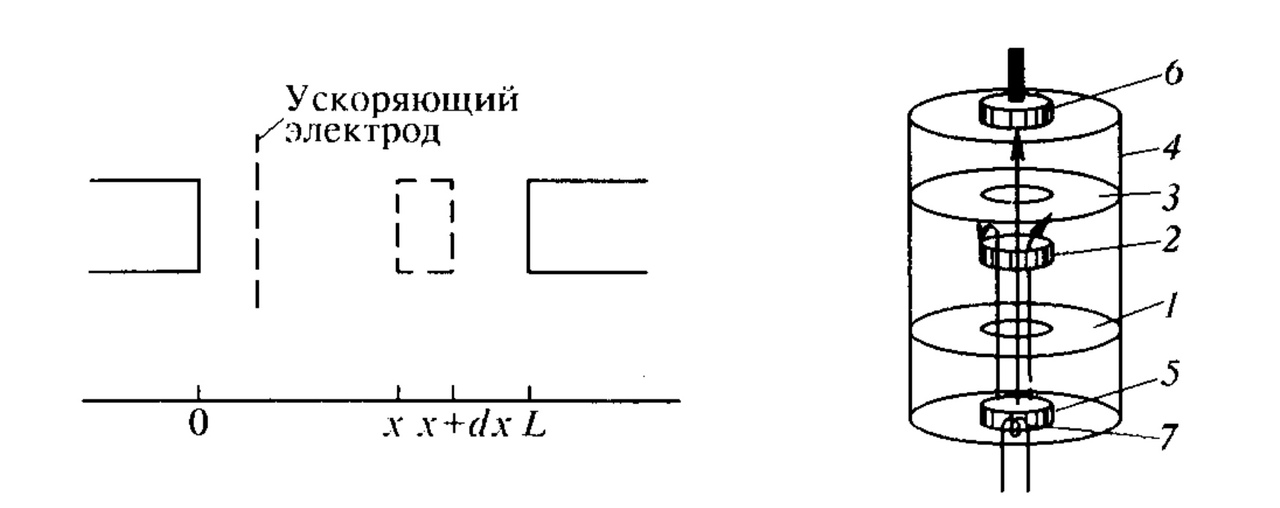
\includegraphics[width=0.7\textwidth]{set.jpg}
    \caption{Схематическое изображение тиратрона (слева) и его конструкции(справа). 1, 2, 3 - сетки, 4 - внешний цилиндр, 5 - катод, 6 - анод, 7 - спираль}
    \label{fig:set}
\end{figure}


\section{Обработка результатов}
\subsection*{Динамический метод}
В таблице представлены измеренные данные для динамического метода.

\begin{table}[H]
	\centering
	\begin{tabular}{|c|c|c|c|}
	\hline
	$U_{\text{накала}}$, В & $V_{max}$, В & $V_{min}$, В & $V_{\text{пробоя}}$, В \\ \hline
	2,927               & 2,8        & 6,8        & 13,0               \\ \hline
	2,504               & 2,6        & 6,6        & 13,0               \\ \hline
	\end{tabular}
\end{table}
Тогда найдём по формуле (6) оценим глубину $U_0$, а по формуле (5) оценим $l$. Занёсем в таблицу.
\begin{table}[H]
	\centering
	\begin{tabular}{|c|c|c|}
	\hline
	$U_\text{накала}$, В & $U_0$, eV & l, Ангстр. \\ \hline
	2,927               & 0,4     & 3,4        \\ \hline
	2,504               & 0,6     & 3,4        \\ \hline
	\end{tabular}
\end{table}

Ионизационный потенциал тогда можно оценить как 

\begin{equation}
	U = U_0 + U_{\text{пробоя}} \approx 13 \text{ В}
\end{equation}
По этому значению можно подтвердить, что в работе использовался ксенон.
\subsection*{Статический метод}
Полученные данные:
\begin{table}[H]
	\centering
	\begin{tabular}{|cc|cc|}
	\hline
	\multicolumn{2}{|c|}{\textbf{U   = 2,974 В}} & \multicolumn{2}{c|}{\textbf{U = 2,527 В}} \\ \hline
	\multicolumn{1}{|c|}{U, В}     & I, e5 A     & \multicolumn{1}{c|}{U, В}    & I, e5 A    \\ \hline
	\multicolumn{1}{|c|}{0}        & 0,08        & \multicolumn{1}{c|}{0}       & 0,1        \\ \hline
	\multicolumn{1}{|c|}{0,78}     & 13,28       & \multicolumn{1}{c|}{0,64}    & 0,6        \\ \hline
	\multicolumn{1}{|c|}{1,42}     & 161,2       & \multicolumn{1}{c|}{1,58}    & 151,1      \\ \hline
	\multicolumn{1}{|c|}{2,1}      & 171,5       & \multicolumn{1}{c|}{1,83}    & 173,1      \\ \hline
	\multicolumn{1}{|c|}{2,5}      & 140,4       & \multicolumn{1}{c|}{2,13}    & 155,8      \\ \hline
	\multicolumn{1}{|c|}{3,2}      & 108,8       & \multicolumn{1}{c|}{3,2}     & 72,8       \\ \hline
	\multicolumn{1}{|c|}{4,1}      & 91          & \multicolumn{1}{c|}{4,2}     & 43,7       \\ \hline
	\multicolumn{1}{|c|}{4,7}      & 83,4        & \multicolumn{1}{c|}{5,2}     & 33,8       \\ \hline
	\multicolumn{1}{|c|}{5,3}      & 80,2        & \multicolumn{1}{c|}{6,1}     & 29,7       \\ \hline
	\multicolumn{1}{|c|}{5,8}      & 79,6        & \multicolumn{1}{c|}{6,9}     & 28,8       \\ \hline
	\multicolumn{1}{|c|}{6,7}      & 83,1        & \multicolumn{1}{c|}{7,6}     & 29,3       \\ \hline
	\multicolumn{1}{|c|}{7,7}      & 93,4        & \multicolumn{1}{c|}{8,6}     & 32,2       \\ \hline
	\multicolumn{1}{|c|}{8,7}      & 114         & \multicolumn{1}{c|}{9,1}     & 35         \\ \hline
	\multicolumn{1}{|c|}{9,3}      & 128         & \multicolumn{1}{c|}{9,8}     & 43,1       \\ \hline
	\multicolumn{1}{|c|}{10,1}     & 167,1       & \multicolumn{1}{c|}{10,5}    & 49,8       \\ \hline
	\end{tabular}
	\end{table}
Проведя аналогиченые вычисления, приведем данные и графики:
\begin{figure}[H]
    \centering
    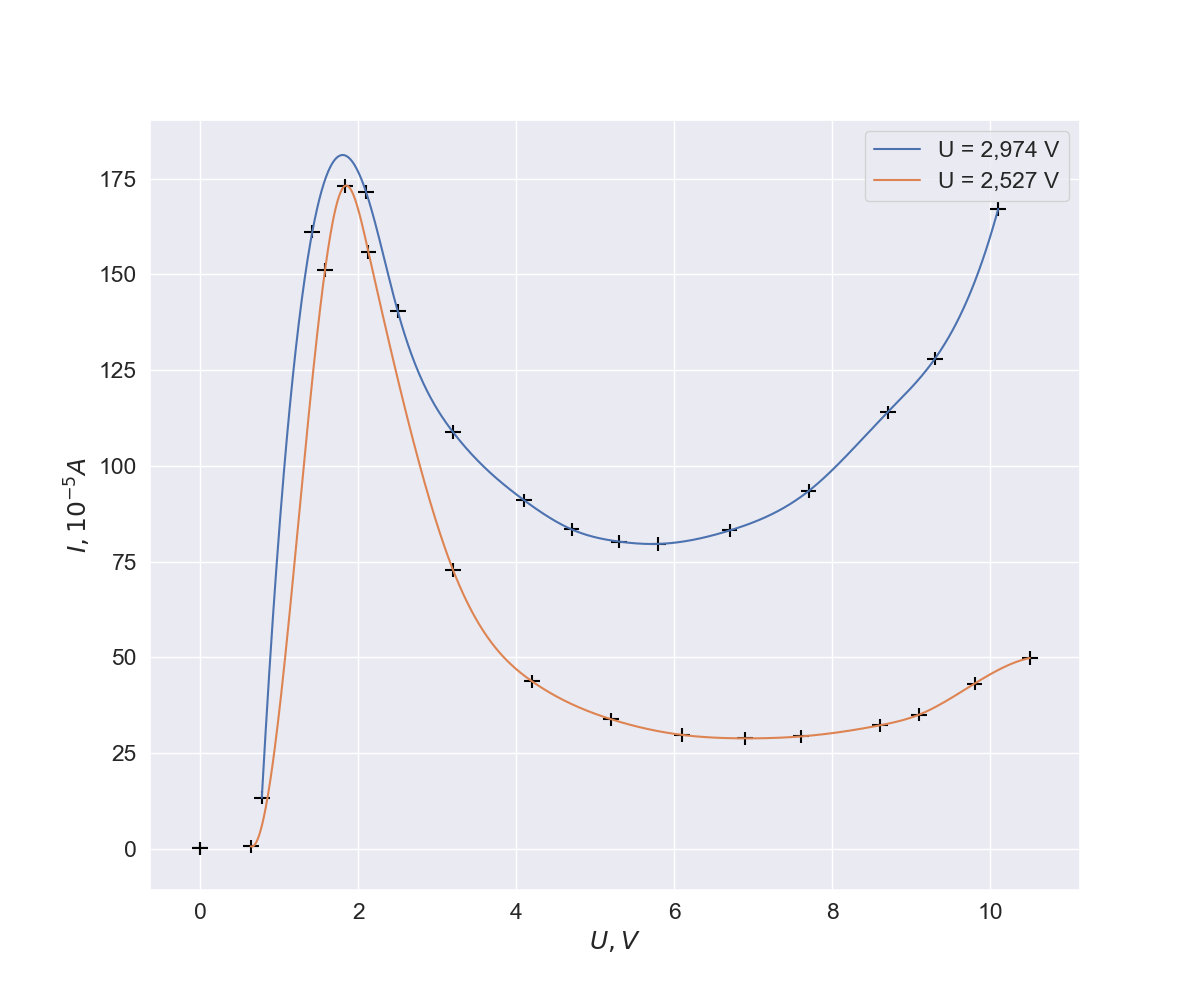
\includegraphics[width=0.8\textwidth]{plot.png}
    \caption{График ВАХ}
    \label{fig:plo1}
\end{figure}

\begin{table}[H]
	\centering
	\begin{tabular}{|c|c|c|}
	\hline
	$U_\text{накала}$, В & $U_0$, eV       & l, Ангстр.    \\ \hline
	2,974               & $1,3 \pm 0,3$ & $3,5 \pm 0,3$ \\ \hline
	2,527               & $2,2 \pm 0,3$ & $3,1 \pm 0,4$ \\ \hline
	\end{tabular}
\end{table}
Далее по формуле \eqref{eq:at} оценим, при каких напряжениях должны появляться максимумы в коэффициенте прохождения электронов:
\[
	E = \sqrt{\frac{\pi n \hbar}{l}} \frac{1}{2 m} - U_0,
\]
Отсюда уже при n = 2 $E > 12 \text{ эВ}$, что больше потенциала ионизации ксенона. Поэтому мы наблюдаем только один максимум.
\section{Выводы}
В результате проведения работы был оценен приблизительный радиус атома ксенона, эффективная глубина потенциальной ямы для электрона. Было подтверждено, что в работе действительно использовался ксенон. В целом работа не очень точная, но статический метод точнее. Динамический позволил получить лишь качественные оценки. В общем, в обоих случаях получилось явно наблюдать эффект Рамзауэра.

\end{document}